\documentclass[../thesis-main.tex]{subfiles}

\begin{document}

\chapter{Computational Methods}
\label{ch:compMethods}

\begin{aquote}{\emph{Hamlet}, Act 2, Scene 2}
  {\fontencoding{T1}\fontfamily{pzc}\selectfont
   Though this be madness, yet there is method in 't.
  }
\end{aquote}
\rule{\linewidth}{0.25mm}

\begin{quote}
 \emph{This chapter presents the computational methods that are used throughout this dissertation---it provides both a summary of those techniques that are used generally throughout this thesis, and also those techniques that are specific to particular chapters. The background to the representation of multidimensional data will be given, with the techniques used explored. The computational models and frameworks used will be expanded upon, and techniques used in their simulation  will be mentioned. Details will be given regarding model adaptation to isch\ae{}mic conditions. The tools used in exploring the parameter space will be explained, and their integration with other models commented upon. Methods used to calculate particular biomarkers used in this dissertation are given. This chapter serves to collate the computational methods used in this dissertation, and analysis based on these methods is found in other chapters.}
\end{quote}

\section{Represention of Multi-Dimensional Data}
\label{subsec:cbdr}
Comprehensive investigation of the effect of variation into multiple different parameters in a model can be thought of as an investigation into a multi-dimensional parameter space: each parameter corresponds to a single dimension. A key problem to be overcome when examining multi-dimensional parameter spaces is how to represent the associated data in a manner that is both meaningful and comprehensible. It is only possible to `directly' map the effect of up to two dimensions on a given marker using a contour plot. As such, to visually represent higher dimensional spaces, without losing any of the data in the space, may be thought of as finding a way to represent these spaces in only two dimensions. The method used here is called \emph{clutter-based dimension reordering}, and has been employed in studying the effect of variation on the electrophysiology of neurons \citep{LeBlanc1990, Peng2004, Peng2005, Taylor2006}.

The key aspect of this is the method used to render higher dimensional spaces in two dimensions, which can be thought of as a form of linear projection. Linear projection, from $n$ dimensions to one or two dimensions, is a relatively simple affair with finite data sets, by rearranging the data, and giving each point in the $n$ dimensional a unique point in a 2 dimensional space that has the same number of points contained within it. This is much like slicing a cube, and placing the resulting squares sequentially next to each other. Here, however, the `slices' can exist in higher dimensions, but continuously slicing the dimensional space iteratively reduces the dimensionality of the space until it can be visualised in two dimensions.

The general form of projection, to give each entry in an $n$ dimensional space (represented by $(x_1,\ldots{},x_n)$) a unique point (represented by $x_i'$) in 1D space, is given by
\begin{equation}
 x_i' = \sum_{i=1}^n\left((x_i-1)\prod_{j=i-1}^i N_j\right) + 1,\label{eq:paramSpace-projection}
\end{equation}
which returns a value between 1 and $N$, where $N$ is the total number of data points; the number of data points in each dimension is given by $N_i$. A two dimensional representation can be constructed by splitting the total number of dimensions in two, and treating each separately as above.

A visual representation of this projection process, ending in a two dimensional space, is given in Fig.~\ref{fig:dim-stack}A---the process thus illustrated is referred to as \emph{dimensional stacking}. In the instance illustrated, two of the conductances being varied are chosen at random ($g_1$ and $g_2$), and with all other parameters set to their minimum value, the effect of the variation of $g_1$ and $g_2$ on a particular output metric of interest is plotted using a contour plot; this is Level 1, and is referred to as the lowest level in the dimensional stack. Next, two other conductances are chosen ($g_3$ and $g_4$), and the original Level 1 plot is repeated for each combination of these two parameters. Each of these plots is arranged in a manner reflecting the variation in $g_3$ and $g_4$ to form Level 2 of the stack, \idest{} the Level 1 plot that has $g_3$ and $g_4$ at their minimum values is at the bottom left of the Level 2 grid, and the Level 1 plot that has $g_3$ and $g_4$ at their maximum values is at the top right of the Level 2 grid. This process was then repeated for the last two conductances.
\begin{figure}
 \centering
 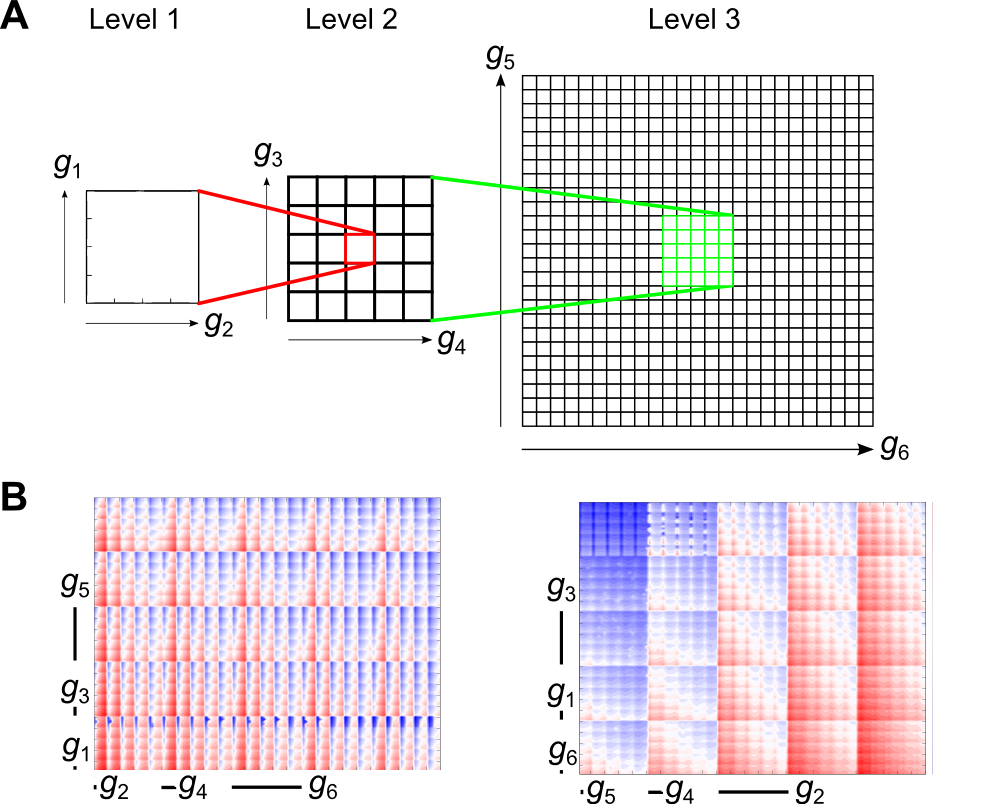
\includegraphics[width=0.75\textwidth]{dimStack}
 \caption[The dimensional stacking process]{(A) The effect of two `low order' conductances ($g_1$ and $g_2$) are plotted in a contour plot, with all other conductances set to their control values. This plot is then embedded in a larger grid spanning two `medium order' conductances ($g_3$ and $g_4$). For each value of $g_{3,4}$, the $g_{1,2}$ plot is repeated for the respective values. This process is repeated to represent the two `high order' conductances ($g_5$ and $g_6$). (B) Example showing a random stack order (left), versus an optimised stack order (right) for the same variable.}
 \label{fig:dim-stack}
\end{figure}

However, the so-called `stack order' (which conductances are plotted as low order and which conductances are plotted as high order) is initially a random choice. The next stage in CBDR is the optimisation of the stack order. This is done by minimising the absolute difference between each point and its four neighbours in the $x$ and $y$ planes; in more general terms, it is those points that are separated by one step in one dimension. An alternative definition of `neighbour' is those that are separated by one step in multiple dimensions---in two dimensions, this would thus include the diagonally connected points. However, \citet{Taylor2006} demonstrated that the connectivity of the space is not adversely affected by using the more restrictive definiton. This will be expanded upon further is \S\ref{subsec:space-connectivity}.
% 
This process of minimisation is done by comparing the score of the current stack order with the score of the neighbouring stack orders (which are those stack orders that are identical save for the swapping of two conductances). If one of the neighbouring stack orders has a lower score than the current stack order, the neighbour's order is adopted, and the process is repeated. While this would technically lead only to a local minima in the stack order space, in practice it is rare for the global minimum to be found (this is confirmed by performing multiple searches, each for a different start order).

The results of such an optimisation process is to `smooth' the image, as shown in Fig.~\ref{fig:dim-stack}B. This means that those parameters with a lesser effect on the measured biomarker are assigned as `lower order' conductances (Level 1), while those that have a greater effect are `higher order' (Level 3). By rearranging the stack order to this optimum stack order, it is thus easier to discern the patterns within the data, both in terms of which parameters have the greatest effect, and also (by virtue of the complete representation of the parameter space) details of the interactions between the parameters.

\section{Computational Models \& Simulation Techniques}
\label{sec:comp-models}
Two models were used in this thesis: both are designed to utilise biophysically detailed formulations of key currents to reproduce the action potential of rabbit epicardial myocytes. The first is presented in \citet{Shannon2004} (henceforth referred to as the Shannon model/framework), and the second is that presented in \citet{Mahajan2008} (or the Mahajan model/framework).\footnote{It should be noted that, according to the previous dominant modelling paradigm, these are individual models. However, as it is one of the main driving forces of this thesis to replace a single model with a population of models, it is useful in the context of this dissertation to think of these two papers as providing \emph{frameworks} on which to base model populations, rather than as individual models.} The Mahajan framework is itself based on the Shannon framework, with alterations made to the L-type \ca{} current, intra\-cellular \ca{} cycling, \na{}-\ca{} exchanger and channel distributions; these alterations were made to allow the model to better fit the provided training data for AP and \ca{}-handling dynamics at rapid pacing rates.

The frameworks for both models were downloaded from the \href{http://models.cellml.org/cellml}{CellML repository} \citep{Lloyd2008}), with the Shannon framework corrected according to \citet{Shannon2012}. These CellML files were then converted to C++ using the \href{http://cor.physiol.ox.ac.uk}{Cellular Open Resource software} \citep{Garny2003, Garny2009}, and all simulations were performed using an ordinary differential equation solver with adaptive time-stepping (\href{http://computation.llnl.gov/casc/sundials/description/description.html}{CVODE}), with relative and absolute tolerances set to $10^{-7}$ and $10^{-9}$, respectively. Both frameworks, in describing the AP of ventricular epicardial myocytes, require stimulation by an external source for the development of an AP. This is provided by a stimulus current (\istim{}), applied appropriately to pace the cell at a given cycle length (CL). This takes the form of a 3 ms step function current, and is initially the same as is provided with the CellML file.

\subsection{Nimrod Distributed Computing Grid}
\label{subsec:nimrod}
While the CVODE solver dramatically reduces simulation time when compared to a Forward Euler ODE solver, when investigating parameter spaces, the sheer number of simulations that have to be run can quickly escalate dramatically. However, parameter space investigation is an embarrassingly parallelisable problem, \idest{} there is no communication between each individual simulation used to investigate the space, and thus, given the correct tools, it is a relatively simple matter to parallelise the search. To this end, the Nimrod/G distributed computing grid \citep{Abramson2000, Abramson2010} is used. Developed by the Monash eScience and Grid Engineering Laboratory, this system permits a correctly written program to be run in parallel across multiple resources. While the use of this tool will be expanded upon only insofar as it furthers the goal of this thesis, it must be remembered that this presents a powerful option for many possible problems \citep{Abramson2011, Abramson2009}.

Of note for this dissertation is the ability to copy an executable program from the `root' to one of several `nodes'---the exact number of nodes available depends entirely on the resources available to user. The results of the simulation are then copied from the node back to the root, and saved according to instructions provided in a given \emph{plan file}, an example of which is given in Code Excerpt~\ref{code:plan-file}. To perform the substitution in the manner described in this way, the executable must be prepared to accept this input---an example of C++ code that produces such an executable is shown in Code Excerpt \ref{code:c++-code}.
\begin{listing}[tb]
 \begin{verbatim}
  parameter x float range from 1 to 10 step 1;

  task main
   copy param-search.exe node:./
   copy param_var.sub node:./
   node:subsitute inputfile.sub inputfile
   node:execute param-search.exe
   copy node:output.dat output.${x}
  endtask
 \end{verbatim}
 \caption[Nimrod/G code: Plan File]{Example of plan file used from the Nimrod `root' to determine Nimrod execution. In this instance, after copying the executable param-search.exe and the substitution file inputfile.sub to the node, the Nimrod/G platform performs the substitution and the exection, before copying the resulting output file output.dat from the node back to the root.}
 \label{code:plan-file}
\end{listing}

\begin{listing}[tb]
 \begin{minted}[gobble=2]{cpp}
  // Declare the file parameter to read the data
  std::ifstream params;
  // Open the file
  params.open("inputfile");
  // Check the file is open
  assert(params.is_open());
  // Push the value that it reads from file into the variables
  params >> x;
 \end{minted}
 \caption[Nimrod/G code: Parameter Substitution]{Excerpt of C++ code required for resulting executable program to be able to perform substitution as per the plan file shown in Code Excerpt~\ref{code:plan-file}.}
 \label{code:c++-code}
\end{listing}

It should be noted that there are many ways to skin a cat, and it is possible to pass parameter values directly to the executable using the appropriate command line syntax.

The Nimrod/G platform is a powerful tool, but it must be remembered that it provides only a tool, and the means of analysis are still within the hands of the user. With regards this thesis, this presents itself in the choice of the parameters being varied. It can be noted from other analyses of variation and variability in \S\ref{subsec:comp-var} that the extent of variation that has been proposed can vary across a huge range. However, in performing the comprehensive parameter sweep proposed in this work the sheer volume of data generated must be borne in mind. To that end, the number of parameters to be varied, and the extent of their variation, is chosen to reflect the best trade-off between:
\begin{itemize}
 \item Resolution of the parameter space,
 \item Breadth of the parameter space,
 \item Number of varied parameters,
 \item Volume of data generated.
\end{itemize}
The volume of data being generated in itself is not an issue \emph{per se}, but rather an indication of how many data can be \emph{usefully} generated. The dimensional stacking mentioned earlier is of use only in so far as the visual representation remains comprehensible---a dimensional stack loses utility when it is not possible to keep some mental track of what the relevance of each parameter is.

% Model adaptation (CellML, C++, simulation time, etc.)
% Nimrod
% Computational tractability, i.e. trade-off between resolution and power/data volume

\subsection{Parameter Space Simulations}
\label{subsec:paramSpace-simulation}
The first stage in this thesis is to (a) examine the effects of simultaneous variation in multiple parameters on model output, and (b) determine which of those models amongst those simulated produce output that matches the experimental literature, thus producing a population of models to reproduce the experimental variation.

Internal \K{} concentration (\ki{}) was unclamped, and variables introduced to alter the peak conductances of six different ion channels (the reasons for varying these parameters specifically will be given in \S\ref{sec:paramSpace-methods}).

The equations representing ion flow through ion channels (and the associated current) is mostly given according to Eq.~\eqref{eq:ion-current}. However, even when the formulation of the model is more complicated, \eg{} a Markov model, an important consideration at this stage is the \emph{compartmentalisation} of the model, which refers to whether there is a spatial subdivision of the ion channel distribution in the cell (see also \S\ref{subsec:model-development}). Both Shannon and Mahajan frameworks are, for the main part, non-compartmentalised models. The reason this is of note here is due to the consequent physiological meaning of altering the peak ion channel conductance ($g_X$). As there is no spatial distinction in the cell model, any changes in $g_X$ can be thought of as a change in (a) the peak conductance of an individual ion channel, or (b) a reduction in the total number of ion channels within the cell; mathematically, the two are equivalent.

Among the ion channel conductances being varied is the for the transient outward current (\ito{}). However, in both Shannon and Mahajan frameworks, \ito{} is composed of two components: a fast and slow activating component (\itof{} and \itos{}, respectively)---for further details, see \S\ref{subsubsec:channel-dynamics}. To thus model variation of \ito{} within these frameworks, a scaling factor not present in either framework was introduced (\gto{}), which was applied to the summation of \itof{} and \itos{}. Individual references to \itof{} and \itos{} (beyond those equations required to directly calculate the current) are not present, and thus replacing references to $(I_\textnormal{to,f}+I_\textnormal{to,s})$ with \ito{} makes no difference to the end result.

The purpose of the simulations examining the parameter space was to elucidate the model's `steady state' behaviour. As such, it was felt that an extended simulation time was appropriate, to allow the model to fully `relax' to the behaviour that would characterise the framework's response to a given parameter set. Initial simulations conducted using COR and the original CellML file of the Mahajan framework indicated that changes to the AP would be complete within 750 s of simulation, given changes in the parameter set that be included in the eventual search. On this basis, initial simulation time was set to 1,000 s, with data recorded for the last two stimulated APs. Each model output was checked for steady state by comparing corresponding data points for the last two data points: the cell was considered to be in steady state if the difference for each data point in the AP was less than $5\%$ of the difference between the maximum and minimum AP values for the last AP. In common with the preliminary tests, steady state was often reached within the initial simulation time. For those models where steady state was not reached, and yet cell excitation was present, simulation was continued until steady state was reached.
% K unclamped
% Simulation duration - reach steady state!
% Physiological effect of varying g_X (decrease channel conductance or number of channels)
% Mention difference with I(Ca,L) for Mahajan model (markov model)
% Form of ito

\subsection{Isch\ae{}mia Simulations}
\label{subsec:isch-simulation}
The model populations determined using the methodology described in the previous cell were entirely appropriate for their task---reproduction of the normal, electrophysiological AP. Consequently, to investigate the changes involved in using model populations in studying isch\ae{}mia, adaptations must be made. As was mentioned in \S\ref{subsec:ischaemia}, much work has been done to allow accurate computational assessment of isch\ae{}mia, and thus the frameworks were adapted to allow the models to reproduce the symptoms of isch\ae{}mia.

The first stage was to define a new `model' model with which to train the new adjustments (the original models were not in the defined populations---for further details, see the results presented in \S\ref{subsec:population-trends}). To this end, the model within the populations that produced the value for APD\sub{90} closest to the population mean at all previously simulated CLs (400 ms, 600 ms and 1,000 ms) was selected. All subsequent single model simulation and analysis was performed using this model (Table \ref{table:isch-model}). Using this new model, the value of \istim{} is then retrained---\citet{Sutton2000} demonstrated the possible important implications for \istim{} on calculated ERP. The new value of \istim{} is designed to be 1.5 times greater than the minimum value that causes cell excitation (after 3 ms application). Finally, the cell is simulated for an extended previous time period, with the resulting model parameters (for such details as ion concentrations) then being fixed. This was done to try and ensure that the population, prior to isch\ae{}mic conditions, would have conditions that would be most appropriate for the defined population, rather than for a model that is no longer included in the population.
\begin{table}
 \centering
 \begin{tabular}{lcccccc}
		& \gto{}	& \gca{}	& \gkr{}	& \gks{}	& \gkix{}	& \gnak{} \\
  \hline
  Shannon	& $+30\%$	& $+0\%$	& $+0\%$	& $-15\%$	& $-30\%$	& $+15\%$ \\
  Mahajan	& $+0\%$	& $+75\%$	& $+30\%$	& $+75\%$	& $+15\%$	& $-30\%$ \\
 \end{tabular}
 \caption[Models used to train isch\ae{}mia conditions]{Details of the variations in given peak ion channel conductances from originally provided values for the model for the Shannon and Mahajan populations that produce APD\sub{90} closest to the population mean for CLs of 400 ms, 600 ms, and 1,000 ms.}
 \label{table:isch-model}
\end{table}

With these considerations complete, the model was subsequently adapted to recreate isch\ae{}mic conditions. The mechanisms used were mostly in common with those from \citet{Rodriguez2006}, with the addition of alterations in the \na{}-handling system of the cell. The changes associated with isch\ae{}mia are summarised in \S\ref{subsubsec:ischaemia-ap}, and are here modelled according to:
\begin{description}
 \item[Anoxia:] Activation of \ikatp{} channels to $0.8\%$ full activation, and inhibition of \inak{} by $30\%$.
 \item[Hyperkal\ae{}mia:] Increase in extracellular \K{} concentration (\ko{}). Associated with this is an increase in \nai{}.
 \item[Acidosis:] Decrease in peak conductance of \ina{} and \ica{} by $f_\textnormal{inhib}=25\%$.
\end{description}
For all conditions, their values are varied independently to allow exploration of the isch\ae{}mic parameter space. In addition to this, the values are varied linearly from their `normal' conditions to their `isch\ae{}mic' conditions to allow approximation of evolution of the population response during isch\ae{}mia; this is in common with \citet{Rodriguez2004}.

The model of \ikatp{} used here is common in its overall structure to that used in \citet{Michailova2007}, itself inherited from \citet{Michailova2005}, and is expressed according to:
\begin{equation}
 I_\textnormal{K-ATP} = f_\textnormal{K-ATP}g_\textnormal{K-ATP}\left(\frac{[\textnormal{K}^+]_\textnormal{o}}{[\textnormal{K}^+]_\textnormal{o,normal}}\right)^{0.24}(V_m-E_\textnormal{K}),
\end{equation}
where \fkatp{} represents the fraction of \ikatp{} channels activated, \gkatp{} represents the peak ion channel conductance and $[\textnormal{K}^+]_\textnormal{o,normal}$ represents the pre-isch\ae{}mic value of \ko{} (which is considered to be 5.4 mM); the other values in the equation are as defined previously. It should be noted that this is a simplified version of the Michailova formulation; for simplicity, terms regarding the regulation of the channel by changing concentrations of ATP and ADP are implicitly included in the value for \gkatp{}.

As has been mentioned in \S\ref{subsubsec:anoxia}, the `spare channel hypothesis' suggests that full activation of \ikatp{} is not necessary, and does not occur, during isch\ae{}mia, with $f_\textnormal{K-ATP}=0.8\%$ being suggested as a reasonable degree of activation. Coupled with this degree of activation is the value assigned to \gkatp{}, which is thus trained to produce a similar value to other forms of the current at equivalent degrees of isch\ae{}mia. Further to this, preliminary analysis was performed to examine the effects of varying values of \gkatp{} on both different models---the results are shown in Fig.~\ref{fig:gkatp-effect}. As can be seen, the models respond differently to the value of \gkatp{} used. On the basis of this result, and in the interests of maintaining consistency with prior work, a value of $g_\textnormal{K-ATP}=2.61$ mS$\mu$F$^{-1}$ was used.% Detail comparison with Sara and Michailova, and effect of changing gkatp (graphs)
\begin{figure}
 \centering
 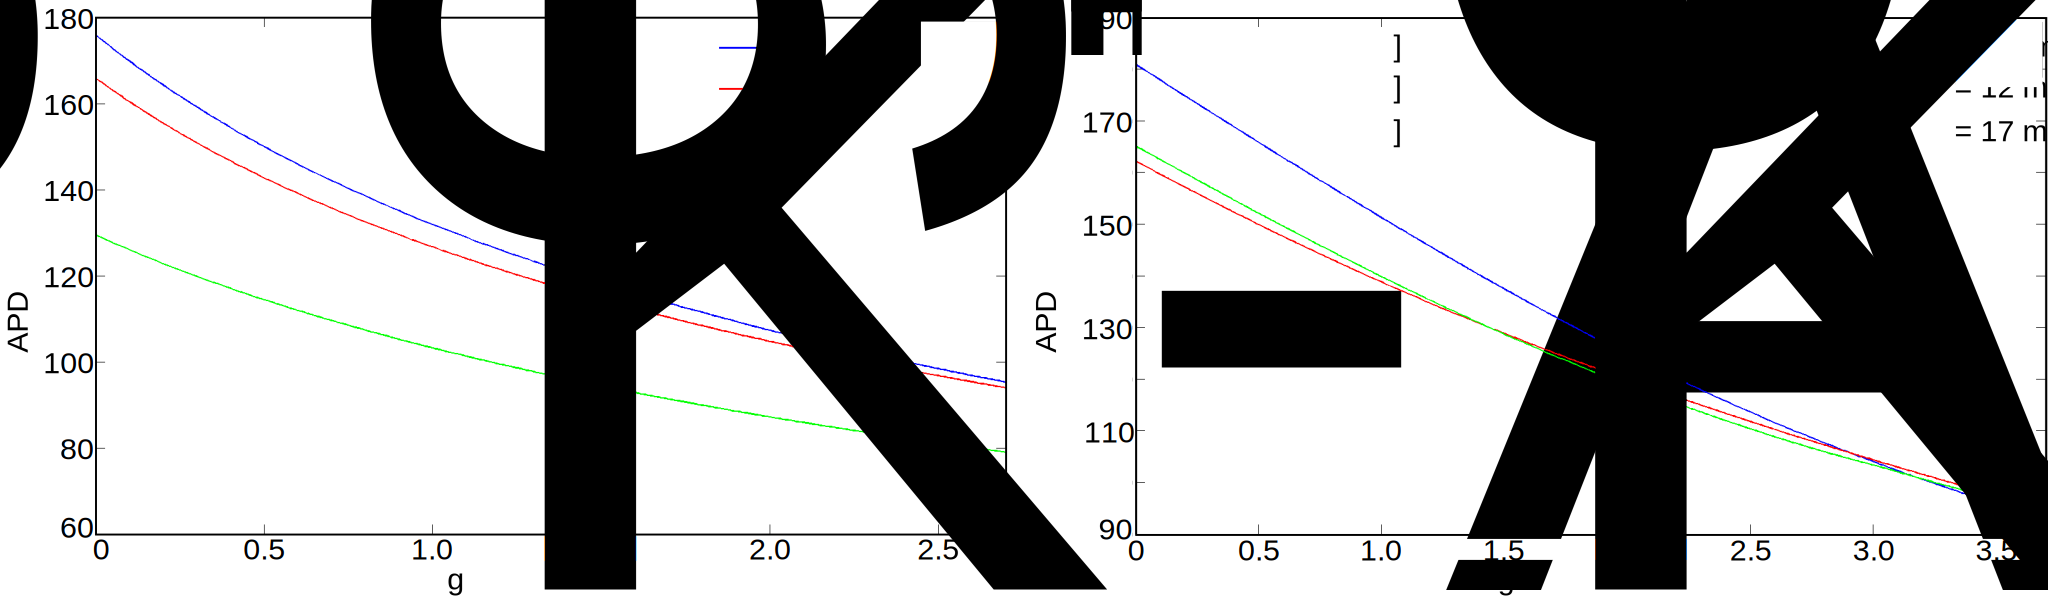
\includegraphics[width=0.85\textwidth]{gkatp-effect}
 \caption[Effect of varying \gkatp{} on APD\sub{90}]{The effect of varying the value of \gkatp{} (with $f_\textnormal{K-ATP}=0.8\%$) on APD\sub{90} for Shannon (A) and Mahajan (B) models. The effect is charted against normal conditions, and two possible isch\ae{}mic concentrations of \ko{}.}
 \label{fig:gkatp-effect}
\end{figure}

The extent of increase in \ko{} due to isch\ae{}mic hyperkal\ae{}mia is subject to debate---prior work tends to put the increase to a value of $\sim12$ mM. However, \ko{} is a remarkably variable quantity, not only with regards its `isch\ae{}mic' value, but also with regards its `normal' value. As such, while $[\textnormal{K}^+]_\textnormal{o,normal}$ is set to 5.4 mM and $[\textnormal{K}^+]_\textnormal{o,isch\ae{}mia}$ is set to 17 mM, the parameter space for \ko{} is also explored.

The value for \nai{} is clamped, and the change (with fully isch\ae{}mic conditions representing a $30\%$ increase) imposed at the start of the simulation. Inhibition of ion currents (\ina{}, \ica{} and \inak{}) is achieved in the same manner as in the earlier parameter space search: direct reduction of the peak conductance $g_X$.

The simulation protocol is to (i) impose the relevant conditions directly to the model, (ii) stimulate the cell at a CL of 600 ms for 10 APs, (iii) record the data for the last AP for subsequent analysis. The model was assessed to be viable if the difference between \vmax{} and \vest{} was greater than 44.0 mV; this value was used based on tests conducting using the Shannon population.

Preliminary simulations with the Shannon model indicated that the broad strokes of the model response are achieved within this timeframe, it can be noted that some models are sensitive to simulation duration, especially within the Mahajan population. However, further simulation time would be misleading: these models, and the changes imposed upon them to reproduce isch\ae{}mia, are approximations, and the models are most suited to short-term simulations---neither model framework is designed to reproduce the complicated effects of the medium- to long-term effects of isch\ae{}mia. As such, the simulation duration is designed to reproduce most faithfully the short-term impacts of isch\ae{}mia.

% Mention importance of Istim, hence importance of making sure it is set correctly
% Simulation duration - difficlties of short/long simulation and temporal effects in modelling ischæmia

\section{Biomarker Calculation}
\label{sec:biomarkers}

Biomarkers represent a means of quantitatively comparing different APs, and with the large volumes of data generated by parameter searches and model populations, a means of automating the analysis of model response is vital. For this reason, biomarkers present a valuable tool to compare data with previous experimental data from the literature. While many biomarkers are common throughout the literature, some are poorly defined. As such, the following defines the terms as used in this dissertation.

\vrest{} is defined as the value of $V_m$ immediately prior to application of \istim{}---due to the lack of any leak current in these models (due to being ventricular myocyte models), this is synonymous with the minimum/diastolic value of $V_m$ during the AP. Similarly, \vmax{} is defined as the maximum value of $V_m$ during the AP. \dvdt{} is the rate of maximum membrane depolarisation, and corresponds to a measure of the rapidity of the upstroke of the AP. It should be noted that \dvdt{} is directly proportional to the square of the conduction velocity of the AP in tissue \citep{Hodgkin1954, Kleber2004, Walton1983, Tasaki1957}.

The plateau membrane potential (\vplat{}) is defined as the point at which \dvdt{} reaches its maximum value (while still remaining greater than 0) after the initial upstroke. Thus, in an AP with a spike and dome morphology, it corresponds to the maximum value of $V_m$ after the initial upstroke. AP duration (APD$_X$) is one of the more common AP biomarkers, but suffers from beign relatively poorly defined, at least to the extent that there can be confusion about the specific definition while the broad strokes of the definition are agreed upon. Here, APD$_X$ is defined as the time interval between the point of \dvdtmax{} and the point at which $V_m$ is repolarised by $X\%$ (\idest{} where $V_m$ is less than or equal to $V_\textnormal{rest}+X(V_\textnormal{max}-V_\textnormal{rest})$.

The effective refactory period (ERP) and post-repolarisation refactoriness (PRR) are also measured, where PRR is defined as ERP$-$APD\sub{90}. In tissue, ERP is defined as the length of time required for the tissue to become excitable after excitation; however, such a definition is not able to be used in ventricular cell models where a stimulus current is applied. As such, the method used to calculate ERP here is the same used used in \citet{Tice2007, Romero2009a, Trenor2007, Pandit2013}, where the time interval between activation and the product of the $h$ and $j$ inactivation gates of \ina{} equalling $0.012$ ($h.j_\textnormal{crit}$) is used as a proxy. This method is used due to the importance of \ina{} during the upstroke of the AP, with the rationale that while \ina{} is still inactivated, the cell can still be regarded as refactory. $h.j_\textnormal{crit}$ is corroborated as being a valid value by confirming that $t(hj_\textnormal{crit}=0.012) \approx t(\textnormal{APD}_\textnormal{90})$ under normal conditions, \idest{} under normal conditions, ERP$\approx$APD\sub{90}.

Biomarkers for \cai{} were also calculated. \casys{} and \cadia{} were the systolic and diastolic values of \cai{}, respectively, and the difference between these two values is referred to as the calcium transient (CaT). Finally, the calcium transient duration (CTD$_X$) was defined in an analagous manner to APD$_X$.

For reasons detailed in the results presented in \S\ref{subsec:biomarker-accuracy}, biomarkers were also required that used the total data available from the AP. To this end, a normalised root mean square deviation measure was defined according to
\begin{equation}
 M_\textnormal{NRMSD} = \frac{1}{M_\textnormal{max}-M_\textnormal{min}}\sqrt{\frac{\sum_{j=1}^N (M_\textnormal{combination}(j)-M_\textnormal{original}(j))^2}{N}}, \label{eq:nrmsd}
\end{equation}
where $M_\textnormal{max}$ and $M_\textnormal{min}$ are the maximum and minimum $V_m$ or \cai{} values for the original model, $M_\textnormal{combination}(j)$ and $M_\textnormal{original}(j)$ are the data points for $V_m$ or \cai{} for a given parameter set and the original model, and $N$ is the number of data points. Importantly, the normalisation step in this equation allowed \aprms{} and \carms{} to be directly compared. By using data from the entire AP or \ca{} transient, this method is a robust measure of goodness-of-fit; however, it is computationally expensive and poorly suited for comparison of model output with noisy experimental data. Furthermore, a comparison using such a metric requires the totality of recorded data to be available for all subsequent comparisons, in contrast to the other biomarkers, where comparison can be made on the basis of a single number.

\biblio

\end{document}